\section{Methods}
\label{sec:methods}
\subsection{Prediction target and error measures}
Let $S=\{s_1,\ldots,s_n\}$ denote the locations of the observed training responses. Write $\widehat m_T(t)$ for the prediction at location $t$ from a prediction model fitted using observations at $T$. The final prediction model uses all observations at $S$; CV fits the same type of prediction model to subsets of these observations.

The target distribution $Q$ specifies where prediction error is evaluated and how errors at those locations are averaged. For a target grid $\{t_1,\ldots,t_M\}$, assign nonnegative weights $q_1,\ldots,q_M$ that sum to one. The squared error at $t_j$ is multiplied by $q_j$ before the errors are added. With equal weights, $q_j=1/M$, so target error is the ordinary average of the errors at the $M$ grid points. This defines error at those points. Using that average to approximate error across an entire region requires a grid and weights that represent the whole region.

For one CV partition, the disjoint test folds $H_1,\ldots,H_K$ together contain all locations in $S$. Fold $f$ trains on a nonempty set $T_f\subseteq S\setminus H_f$ and predicts the responses at $H_f$. Ordinary CV uses $T_f=S\setminus H_f$ \citep{arlot2010survey}. With buffering, observations within a specified distance of any test location are also removed from that fold's training set. This changes the training set while leaving its test fold unchanged. Each observation therefore supplies one held-out prediction, and the observed CV MSE (the CV score) $\widehat C$ is the average of the resulting $n$ squared errors:
\[
 \widehat C=\frac{1}{n}\sum_f\sum_{i\in H_f}[Y(s_i)-\widehat m_{T_f}(s_i)]^2.
\]
Thus each test observation contributes with weight $1/n$, even when the folds have different sizes.

MSE, or \emph{risk}, is the expected squared difference between a response and its prediction. Here, $\E_Y$ averages over possible datasets of training and target responses from the same spatial model, including observation noise. Prediction models are refitted for each dataset. Locations, target weights and CV folds are chosen without using response values and held fixed.

At a target location, $Y(t)$ denotes the response to be predicted, including observation noise. If a target location coincides with a training location, it represents a new measurement with independent observation noise. Define the target MSE $R_Q$, expected CV MSE $C$, and their difference $O$ as
\begin{align}
 R_Q &= \E_Y\E_{t\sim Q}\{[Y(t)-\widehat m_S(t)]^2\},\\
 C &= \E_Y(\widehat C),\qquad O=R_Q-C.\label{eq:risk}
\end{align}
Here $\E_{t\sim Q}$ averages over target locations; on a finite grid, it weights the error at $t_j$ by $q_j$. A positive $O$ means that CV underestimates target MSE on average, and a negative $O$ means that it overestimates it. We call $O$ \emph{optimism}; the usual estimator bias is $C-R_Q=-O$. The difference reflects both the locations used for validation and the smaller training sets used within CV.

For a particular observed dataset, the relevant target MSE keeps its training responses $Y_S$ and fitted prediction model fixed, and averages over possible target responses conditional on $Y_S$ \citep{bates2024crossvalidation}. Denote this conditional target MSE by
\[
 R_Q(Y_S)=\E_{t\sim Q}\E\bigl\{[Y(t)-\widehat m_S(t)]^2\mid Y_S\bigr\}.
\]
The difference $R_Q(Y_S)-\widehat C$ measures the error of that dataset's CV estimate. A small $|O|$ can coexist with large errors for individual datasets, because underestimation in some datasets can cancel overestimation in others.

The known-covariance experiment calculates $O$ analytically and compares selection rules using the average of $|O|$ across location configurations. The experiment with estimated covariance instead calculates $|R_Q(Y_S)-\widehat C|$ for each simulated dataset and averages these absolute errors. It therefore assesses how accurately the observed CV MSE estimates the conditional target MSE of the prediction model fitted to that dataset.

\subsection{Nearest-neighbour distance distributions}
\label{sec:distances}
Following nearest-neighbour distance matching \citep{mila2022nndm,linnenbrink2024knndm}, we compare validation and target nearest-training distances. For each validation observation at $s_i\in H_f$, define its nearest-training distance as
\[
 d_i^C=\min_{s\in T_f}\|s_i-s\|,
\]
where $\|s_i-s\|$ is the Euclidean distance between the two locations. The distance is measured from the validation location $s_i$ to the nearest observation available in its fold's training set $T_f$. The search excludes all observations in the test fold and any observations removed by the buffer. This gives one distance $d_i^C$ for each of the $n$ validation observations.

Let $D_C$ denote the distance obtained by choosing one validation observation uniformly from these $n$ observations. Thus $d_i^C$ is the distance for a particular observation, while $D_C$ describes the variation in these distances across validation observations, each with weight $1/n$. The calculation starts from each validation location; starting from each training location and finding its nearest validation observation would define a different distribution.

For each target grid point $t_j$, define
\[
 d_j^Q=\min_{s\in S}\|t_j-s\|.
\]
This is the distance from $t_j$ to its nearest observation in the full training set $S$. Let $D_Q$ denote this distance for a target location drawn from $Q$. On a finite target grid, location $t_j$ contributes its distance $d_j^Q$ with weight $q_j$. With equal target weights, each of the $M$ locations has weight $1/M$.

Let $F_C(u)=\Pr(D_C\leq u)$ and $F_Q(u)=\Pr(D_Q\leq u)$ be the cumulative distribution functions (CDFs). Here $F_C(u)$ is the proportion of validation observations whose nearest available training observation is at most distance $u$ away. On a finite target grid, $F_Q(u)$ is the sum of the weights $q_j$ for target locations whose nearest observation in $S$ is at most distance $u$ away. With equal weights, this is the proportion of target locations satisfying that condition. Figure~\ref{fig:diagnostic}A shows an example set of observation and target locations; Figure~\ref{fig:diagnostic}B compares their distance CDFs under random and blocked CV.

For finite mean distances, two useful summaries are
\begin{equation}
 A=\E D_Q-\E D_C=\int_0^\infty(F_C-F_Q)\,du,\qquad
 W=\int_0^\infty|F_C-F_Q|\,du.\label{eq:geometry}
\end{equation}
The expectations here average distances over validation observations or target locations, using their respective weights. The mean-distance difference $A$ is positive when target locations are farther from training observations on average. The Wasserstein distance $W$ measures the total area between the two CDFs \citep{panaretos2019wasserstein}. It is zero only when the distance distributions match. Both quantities have distance units.

The distinction between $A$ and $W$ becomes important when the CDFs cross. Positive and negative values of $F_C-F_Q$ can cancel in $A$, whereas their absolute values add to $W$. Consequently, equal mean distances can conceal different distributions. In general, $|A|\leq W$; equality holds when the CDF difference has the same sign almost everywhere.

\subsection{Correlation model and contrasts}
\label{sec:correlation-model}
The distance distributions describe how close validation and target locations are to training observations. To describe the strength of dependence at these distances, we use a Gaussian spatial model with independent observation noise \citep[Chapter~2]{rasmussen2006gpml}. Consider
\[
 Y(s)=\mu(s)+Z(s)+\epsilon(s),
\]
where $\mu(s)$ is a known mean and $Z(s)$ is a mean-zero, stationary, isotropic Gaussian spatial process with variance $\sigma^2$ and correlation function $r(u)$. Its covariance depends only on the separation distance $u$. The observation noise $\epsilon(s)$ is mean-zero Gaussian with variance $\tau^2$, independent between measurements and independent of $Z$. Each response therefore has total variance $V=\sigma^2+\tau^2>0$.

For two distinct measurements separated by distance $u$, the covariance is $\sigma^2r(u)$ because the independent noise contributes no covariance. Their correlation is consequently
\[
 \rho(u)=\frac{\sigma^2r(u)}{\sigma^2+\tau^2}=wr(u),
 \qquad w=\frac{\sigma^2}{V}.
\]
Here $r(u)$ is the correlation within the spatial process, whereas $\rho(u)$ is the correlation between the observed responses, including noise. The fraction $w$ is the proportion of response variance attributable to the spatial process. These parameters may be specified in a simulation or estimated from training responses.

For exponential spatial correlation, $r(u)=\exp(-u/\phi)$ and $\rho(u)=w\exp(-u/\phi)$, where $\phi>0$ is a distance scale. At $u=\phi$, the correlation within the spatial process is $r(\phi)=\exp(-1)\approx0.368$. The correlation between observed responses is $\rho(\phi)=w\exp(-1)\approx0.368w$. Larger values of $\phi$ give slower decay; the exponential spatial correlation remains positive at every finite distance. For distinct measurements at the same location, $\rho(0)=w$ because their observation noise is independent. A measurement's correlation with itself is one; the target response here is a separate measurement even when its location coincides with a training location.

We apply the same function $\rho$ to the validation and target distances. The quantities $\rho(D_C)$ and $\rho(D_Q)$ are the correlations implied by this model between a response and its nearest available training response during validation and target prediction, respectively. Their expectations average over the distance distributions defined above, with the correlation function held fixed.

Using the individual distances defined in Section~\ref{sec:distances}, $\rho(d_i^C)$ is the correlation between validation response $Y(s_i)$ and its nearest training response in $T_f$. Similarly, $\rho(d_j^Q)$ is the correlation between the target response at $t_j$ and its nearest training response in $S$. Their averages are
\[
\begin{aligned}
 \E\{\rho(D_C)\}&=\frac{1}{n}\sum_{i=1}^n \rho(d_i^C),
 &\E\{\rho(D_Q)\}&=\sum_{j=1}^M q_j \rho(d_j^Q),\\[4pt]
 \E\{[\rho(D_C)]^2\}&=\frac{1}{n}\sum_{i=1}^n [\rho(d_i^C)]^2,
 &\E\{[\rho(D_Q)]^2\}&=\sum_{j=1}^M q_j[\rho(d_j^Q)]^2.
\end{aligned}
\]
The first row gives the average correlation during validation and at the target. The second row squares each correlation before averaging. Validation observations have equal weights $1/n$; target locations use the weights $q_j$ specified by $Q$. For equally weighted target locations, $q_j=1/M$.

We define the \emph{correlation contrasts} as the differences between the corresponding validation and target averages:
\begin{equation}
 J_1=\E\{\rho(D_C)\}-\E\{\rho(D_Q)\},\qquad
 J_2=\E\{[\rho(D_C)]^2\}-\E\{[\rho(D_Q)]^2\}.\label{eq:indices}
\end{equation}
Both contrasts are dimensionless. A positive $J_2$ means that the average squared correlation with the nearest available training response is higher for validation observations than for target locations. A negative $J_2$ means that this average is higher for target locations than for validation observations. A value of zero means that the two averages are equal. The same sign interpretation applies to $J_1$ using correlations rather than squared correlations. The squared form is motivated by the connection to MSE derived in Section~\ref{sec:one-neighbour} for Gaussian prediction using one neighbour with known mean and covariance.

\subsection{Correlation weighting and distance matching}
The correlation contrasts can also be written in terms of the distance CDFs. This shows how they differ from the Wasserstein distance $W$. For the exponential response correlation $\rho(u)=w\exp(-u/\phi)$, integration by parts gives
\begin{equation}
\begin{aligned}
 J_2&=\int_0^\infty\lambda_2(u)\{F_C(u)-F_Q(u)\}\,du,\\
 \lambda_2(u)&=-\frac{d}{du}[\rho(u)^2]
 =\frac{2w^2}{\phi}\exp(-2u/\phi).
\end{aligned}
\label{eq:weighting}
\end{equation}
The weight $\lambda_2(u)$ measures how rapidly squared correlation decreases with distance. For the exponential model with $w>0$, it is largest at short distances and decreases as $u$ increases. Differences between the two CDFs therefore receive more weight at short distances. This is what we mean by \emph{correlation weighting}. Figure~\ref{fig:diagnostic}C shows the weights for $J_1$ and $J_2$.

A CV scheme specifies the test folds and their training sets. We compare schemes by choosing the smallest $W$ or $|J_2|$. The distance $W$ adds absolute CDF differences equally per unit distance; $J_2$ adds signed differences weighted by $\lambda_2(u)$. When the CDFs cross, positive and negative contributions can offset one another: \emph{cancellation}. Taking the absolute value after integration preserves this cancellation. The two criteria therefore differ in both weighting and cancellation; a small $|J_2|$ need not mean similar distance distributions.

To examine weighting without cancellation, we also evaluate
\[
 U_2=\int_0^\infty\lambda_2(u)|F_C(u)-F_Q(u)|\,du.
\]
This measure uses the same weights as $J_2$ but takes absolute differences before adding them. It is the Wasserstein distance between the distributions of squared correlations, $[\rho(D_C)]^2$ and $[\rho(D_Q)]^2$. The corresponding measure $U_1$ compares the distributions of unsquared correlations. Both measures are nonnegative and satisfy $|J_p|\leq U_p$ for $p=1,2$; the supplementary material (Section~\ref*{supp-sec:transport}) gives their general integral expressions.

Weak spatial signal can make the contrasts small even when validation and target distance distributions differ substantially. For a fixed spatial correlation function $r$ shared by all CV schemes, their common signal fraction $w>0$ scales every $J_p$ by $w^p$. Reducing $w$ therefore shrinks the contrasts without changing which scheme has the smallest $|J_p|$.

\begin{figure}[p]
\centering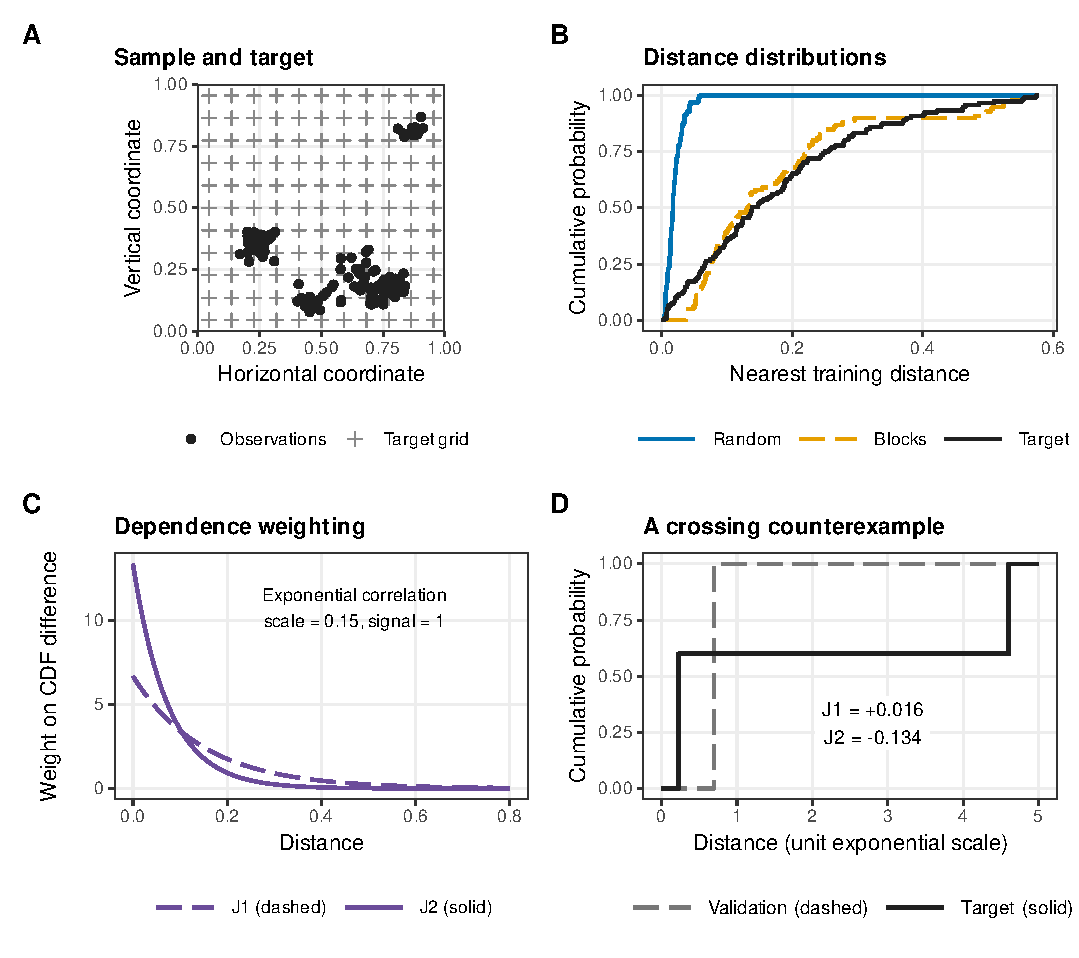
\includegraphics[width=\textwidth]{F1-diagnostic.pdf}
\caption{From nearest-training distances to correlation contrasts. (A) Example observation locations (black circles) and target grid (grey crosses). (B) Distance CDFs for random CV (blue solid), blocked CV (orange dashed) and target prediction (black solid). (C) Weights applied to the CDF difference for $J_1$ (dashed) and $J_2$ (solid), using exponential scale $0.15$ and signal fraction one. (D) A separate example in which the validation CDF (grey dashed) and target CDF (black solid) cross, giving $J_1$ and $J_2$ opposite signs. Panels C and D illustrate specified correlation functions; they do not estimate covariance from panel A. Panel D uses unit exponential scale.}
\label{fig:diagnostic}
\end{figure}

\clearpage
\subsection{Exact MSE difference for prediction using one neighbour}
\label{sec:one-neighbour}
The squared contrast $J_2$ gives an exact MSE difference when prediction uses only the nearest training response. Assume the Gaussian model in Section~\ref{sec:correlation-model}, with known mean and covariance and the same observation-noise variance at training and target locations. If the nearest training response is at $s_*$, a distance $D$ from $t$, Gaussian conditioning gives the prediction that minimises MSE \citep[Chapter~2]{rasmussen2006gpml}:
\[
 \widehat m_T(t)=\mu(t)+\rho(D)\{Y(s_*)-\mu(s_*)\}.
\]
The neighbour's departure from its mean adjusts the mean at $t$, in proportion to their response correlation. The MSE is $V\{1-\rho(D)^2\}$: squared correlation determines how much the neighbour reduces prediction error.

Averaging over target distances gives $V[1-\E\{\rho(D_Q)^2\}]$; averaging over validation distances gives $V[1-\E\{\rho(D_C)^2\}]$. Subtracting expected CV MSE from target MSE therefore gives
\begin{equation}
 O_1=VJ_2.\label{eq:one}
\end{equation}
Here $O_1$ is the optimism defined in equation~\eqref{eq:risk} for this one-neighbour prediction model. Positive $J_2$ means that CV underestimates target MSE; negative $J_2$ means that it overestimates it. Under these assumptions, choosing the CV scheme with the smallest $|J_2|$ also minimises $|O_1|$. These MSEs average over possible training and target responses while keeping locations, folds and target weights fixed. Adding $VJ_2$ removes the average bias of CV under this one-neighbour model. For an individual dataset, the adjusted score can still overestimate or underestimate the fitted model's conditional target MSE.

The distance CDFs can also establish the sign. Suppose response correlation is nonnegative and does not increase with distance. If $F_C(u)\geq F_Q(u)$ for every $u$, validation observations are at least as likely as target locations to have a training neighbour within any specified distance. Then $J_1,J_2,O_1\geq0$: CV underestimates target MSE or equals it. Reversing the CDF ordering reverses the inequalities. Different distance distributions can still give equality where correlation is constant, including when there is no spatial signal.

When the CDFs cross, $J_1$ and $J_2$ can have opposite signs (Figure~\ref{fig:diagnostic}D). Let $m_C,m_Q$ be the means of the validation and target correlations, and $v_C,v_Q$ their variances. Then
\begin{equation}
 J_2=(m_C+m_Q)J_1+v_C-v_Q.\label{eq:moments}
\end{equation}
Thus $J_1$ compares average correlations but omits their difference in variance. For example, suppose validation correlation is always $0.5$, while target correlation is $0.8$ with probability $0.6$ and $0.01$ otherwise. These values are possible under an exponential model and give $J_1=0.016$ but $J_2=-0.13404$. Despite positive $J_1$, CV overestimates target MSE in this example because $O_1=VJ_2<0$.



\subsection{Prediction using all available training observations}
The remaining training observations can supply information beyond the nearest neighbour. Under the same Gaussian model with known mean and covariance, the optimal prediction using all available training observations is simple kriging. Let $Y_T$ be the vector of responses at training locations $T$, $\Sigma_T=\Cov(Y_T)$ their covariance matrix, and $b(t,T)=\Cov(Y_T,Y(t))$ the vector of their covariances with the response to be predicted. If $\Sigma_T$ is nonsingular, the MSE is $V-e(t,T)$, where
\[
 e(t,T)=b(t,T)^\top\Sigma_T^{-1}b(t,T).
\]
Thus $e(t,T)$ is the reduction in MSE supplied jointly by the training observations \citep{rasmussen2006gpml}. Positive observation-noise variance is sufficient for $\Sigma_T$ to be nonsingular.

Let $D(t,T)$ be the nearest distance from $t$ to $T$. Using only that nearest observation reduces MSE by $V\rho[D(t,T)]^2$. The additional reduction supplied by the remaining observations is therefore
\[
 a(t,T)=e(t,T)-V\rho[D(t,T)]^2\geq0.
\]
This quantity is nonnegative because the optimal prediction using all observations could always assign zero weight to the others and reproduce the one-neighbour prediction.

For validation, denote the average total MSE reduction by $\overline{e}_C$ and the average additional reduction beyond the nearest neighbour by $\overline{a}_C$. Each observation has weight $1/n$ and is evaluated using its fold's training set. The corresponding target averages, $\E_Q e(t,S)$ and $\E_Q a(t,S)$, use the target weights in $Q$ and all training observations at $S$.

Expected CV MSE is $V-\overline{e}_C$, and target MSE is $V-\E_Q e(t,S)$. Subtracting expected CV MSE from target MSE cancels the common variance $V$, giving
\begin{equation}
\begin{aligned}
 O_{\mathrm{full}}&=\overline e_C-\E_Q e(t,S)\\
 &=VJ_2+\overline a_C-\E_Q a(t,S).
\end{aligned}
\label{eq:remainder}
\end{equation}
The first term, $VJ_2$, is the MSE difference for prediction using only the nearest neighbour. The remainder, $\overline{a}_C-\E_Q a(t,S)$, measures how much more the other observations reduce MSE during validation than at the target. A positive remainder increases optimism; a negative remainder decreases it. Thus $VJ_2$ alone gives the full MSE difference only when these additional benefits are equal on average.

Matching nearest distances can still leave CV biased. Place observations at $-1$, $0$ and $1$ on a line, and predict at $2$. Leave-one-out CV predicts each observation from the other two; target prediction uses all three. All nearest-training distances are one, so $W=J_1=J_2=0$. When predicting the held-out observation at $0$, both training observations are one unit away. At the target location $2$, only one training observation is one unit away; the others are two and three units away. With $V=1$, $w=0.8$ and $r(u)=\exp(-u)$, these additional neighbours reduce MSE more during validation, on average, than at the target. Thus $O_{\mathrm{full}}=\NeighbourCounterexample>0$: expected CV MSE is lower than target MSE. The difference comes entirely from the additional-neighbour term in equation~\eqref{eq:remainder}; the supplementary material (Section~\ref*{supp-sec:counterexample}) gives the calculation.

\subsection{Bounding the contribution of the other neighbours}
A bound on the additional MSE reduction $a(t,T)$ limits how far the full MSE difference can depart from $VJ_2$. We retain the Gaussian model with known mean and covariance.

Let $Y_1$ be the nearest training response and $Y_R$ the vector of remaining training responses. Write $b_1=\Cov(Y_1,Y(t))$, $b_R=\Cov(Y_R,Y(t))$ and $\Sigma_{R1}=\Cov(Y_R,Y_1)$. Then $\widetilde b_R=b_R-\Sigma_{R1}b_1/V$ contains the covariances between $Y_R$ and $Y(t)$ after conditioning on $Y_1$ \citep[Appendix~A.2]{rasmussen2006gpml}: the dependence remaining once the nearest response is known. For positive observation-noise variance, $\tau^2>0$,
\begin{equation}
 0\leq a(t,T)\leq B(t,T)
 =\min\{\|\widetilde b_R\|^2/\tau^2,\ \sigma^2-b_1^2/V\}.\label{eq:extra-bound}
\end{equation}
Here $\|\widetilde b_R\|^2$ is the sum of the squared entries of $\widetilde b_R$. The first upper bound follows because the remaining observations retain independent noise with variance $\tau^2$. The second is the spatial variance left after the nearest observation has reduced MSE by $b_1^2/V$; independent target noise cannot be predicted. Both limits apply, so $B$ takes the smaller one. The supplementary material (Sections~\ref*{supp-sec:bound-residuals}--\ref*{supp-sec:bound-signal}) gives the pointwise proof.

Let $\overline{B}_C$ be the validation average of $B$, with each observation weighted by $1/n$ and evaluated using its fold's training set. The target average uses $Q$ and the full set $S$. In equation~\eqref{eq:remainder}, the additional validation reduction is added to $VJ_2$, while the additional target reduction is subtracted. Averaging these bounds (supplementary material, Section~\ref*{supp-sec:bound-averaging}) gives
\begin{equation}
 VJ_2-\E_Q B(t,S)\leq O_{\mathrm{full}}
 \leq VJ_2+\overline B_C.\label{eq:certificate}
\end{equation}
A positive lower limit guarantees that CV underestimates target MSE on average; a negative upper limit guarantees overestimation. If the interval includes zero, it does not establish a nonzero bias. These are deterministic limits under the known covariance model, rather than a confidence interval. Computing $B$ requires covariances involving all training observations, beyond the nearest distances alone.

For other prediction models, ordered distance distributions imply an MSE ordering only under additional conditions. One sufficient condition is that MSE does not decrease as nearest distance increases, following the same function during validation and target prediction (supplementary material, Section~\ref*{supp-sec:extensions}). Sections~\ref{sec:sim-covariance} and~\ref{sec:sim-learners} examine the effects of covariance estimation, training size and prediction model; Section~\ref{sec:sim-refitting} tests selection by $|J_2|$ when covariance is estimated.

\subsection{CV schemes and selection rules}
\label{sec:cv-selection}
Each CV scheme defines test folds and their training sets. We compare four candidates, each with five folds. Balanced random folds assign observations randomly to groups of nearly equal size \citep{arlot2010survey}. Spatial blocks use coordinate $k$-means \citep{hartigan1979kmeans} to form geographic groups. Buffered spatial blocks retain the same test folds but remove training observations within the specified buffer distance of any test observation \citep{roberts2017cross}. kNNDM, implemented in CAST 1.1.1, constructs folds to bring validation and target nearest-training distance distributions closer together \citep{linnenbrink2024knndm}. These fold constructions use locations alone. The final prediction model is fitted to all available training observations.

A selection rule chooses among these four candidates using one diagnostic. For each simulation dataset or location configuration, we calculate the diagnostic for every candidate. Selection by $A$, $J_1$ or $J_2$ chooses the smallest absolute value; selection by $W$, $U_1$ or $U_2$ chooses the smallest value. When correlation is estimated for selection, all candidates use the same full-data estimate (Section~\ref{sec:sim-refitting}). The selected scheme supplies the CV estimate of target MSE. We also evaluate two fixed choices: random CV for every dataset and kNNDM for every dataset. These comparisons test whether selecting among schemes improves the CV estimate of target MSE.

In the known-covariance study (Section~\ref{sec:sim-known}), we assess the selected scheme by its absolute expected bias, $|O|=|R_Q-C|$. In the covariance-refitting study (Section~\ref{sec:sim-refitting}), we use \mbox{$|R_Q(Y_S)-\widehat C|$}: the absolute difference between the observed CV score and the conditional target MSE of the model fitted to that dataset.

Candidates whose selection criterion values are within $10^{-12}$ of the minimum are treated as tied. We calculate the absolute error defined above separately for each tied scheme, then average these errors with equal weights. If two schemes tie, each contributes half of its absolute error to this average. Target MSE is used only to assess accuracy; the diagnostic values determine which schemes are selected. The supplementary material (Section~\ref*{supp-sec:uncertainty}) reports checks of the numerical tolerance used to identify ties.
